\hypertarget{interfaceData}{
\section{Data  Interface Reference}
\label{interfaceData}\index{Data@{Data}}
}
Inheritance diagram for Data:\begin{figure}[H]
\begin{center}
\leavevmode
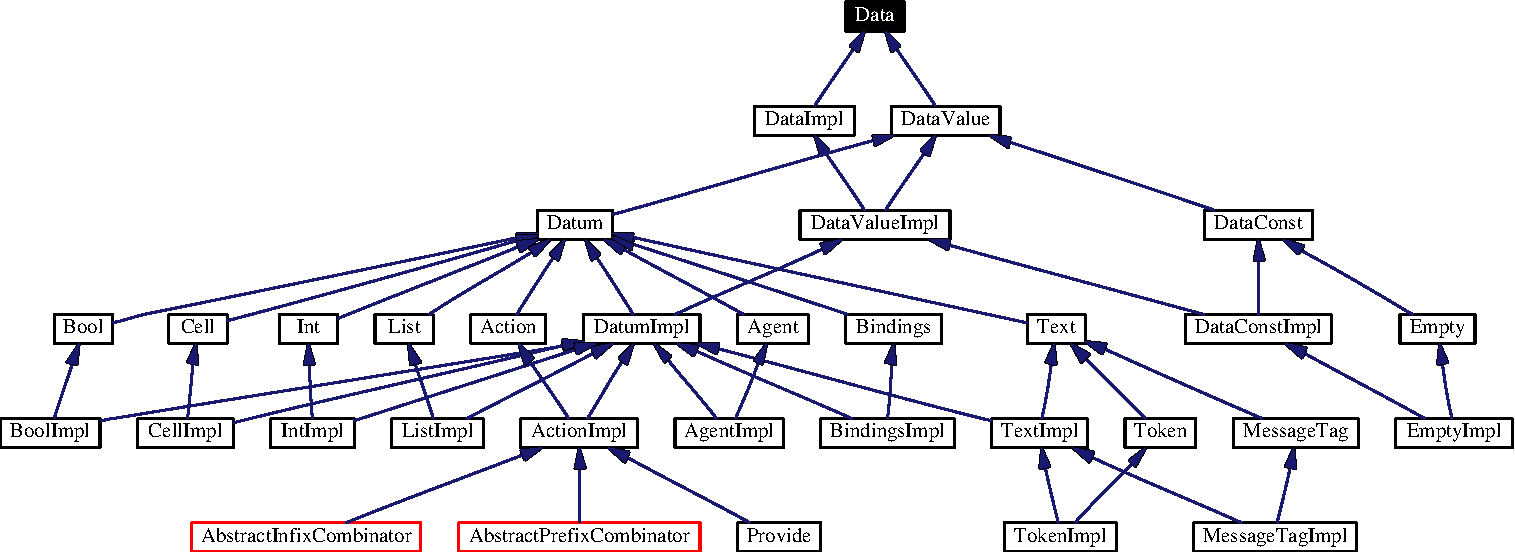
\includegraphics[width=381pt]{interfaceData__inherit__graph}
\end{center}
\end{figure}
\subsection*{Public Methods}
\begin{CompactItemize}
\item 
Data \hyperlink{interfaceData_a0}{concat} (Data data)
\item 
\hyperlink{interfaceList}{List} \hyperlink{interfaceData_a1}{tuple\-To\-List} ()
\item 
\hyperlink{interfaceDataValue}{Data\-Value} \hyperlink{interfaceData_a2}{first} () throws \hyperlink{classExceptional}{Exceptional}
\item 
Data \hyperlink{interfaceData_a3}{rest} ()
\item 
\hyperlink{interfaceDataValue}{Data\-Value} \hyperlink{interfaceData_a4}{at} (int n) throws \hyperlink{classExceptional}{Exceptional}
\item 
\hyperlink{interfaceAction}{Action} \hyperlink{interfaceData_a5}{provide} ()
\end{CompactItemize}


\subsection{Member Function Documentation}
\hypertarget{interfaceData_a4}{
\index{Data@{Data}!at@{at}}
\index{at@{at}!Data@{Data}}
\subsubsection[at]{\setlength{\rightskip}{0pt plus 5cm}\hyperlink{interfaceDataValue}{Data\-Value} Data::at (int {\em n})}}
\label{interfaceData_a4}




Reimplemented in \hyperlink{classDataImpl_a4}{Data\-Impl}, \hyperlink{classDataValueImpl_a4}{Data\-Value\-Impl}, and \hyperlink{classEmptyImpl_a0}{Empty\-Impl}.

Referenced by Data\-Impl::at().

\hypertarget{interfaceData_a0}{
\index{Data@{Data}!concat@{concat}}
\index{concat@{concat}!Data@{Data}}
\subsubsection[concat]{\setlength{\rightskip}{0pt plus 5cm}Data Data::concat (Data {\em data})}}
\label{interfaceData_a0}




Reimplemented in \hyperlink{classDataImpl_a0}{Data\-Impl}, \hyperlink{classDataValueImpl_a3}{Data\-Value\-Impl}, and \hyperlink{classEmptyImpl_a2}{Empty\-Impl}.

Referenced by Data\-Impl::concat().

\hypertarget{interfaceData_a2}{
\index{Data@{Data}!first@{first}}
\index{first@{first}!Data@{Data}}
\subsubsection[first]{\setlength{\rightskip}{0pt plus 5cm}\hyperlink{interfaceDataValue}{Data\-Value} Data::first ()}}
\label{interfaceData_a2}




Reimplemented in \hyperlink{classDataImpl_a2}{Data\-Impl}, \hyperlink{classDataValueImpl_a0}{Data\-Value\-Impl}, and \hyperlink{classEmptyImpl_a1}{Empty\-Impl}.\hypertarget{interfaceData_a5}{
\index{Data@{Data}!provide@{provide}}
\index{provide@{provide}!Data@{Data}}
\subsubsection[provide]{\setlength{\rightskip}{0pt plus 5cm}\hyperlink{interfaceAction}{Action} Data::provide ()}}
\label{interfaceData_a5}




Reimplemented in \hyperlink{classDataImpl_a5}{Data\-Impl}.\hypertarget{interfaceData_a3}{
\index{Data@{Data}!rest@{rest}}
\index{rest@{rest}!Data@{Data}}
\subsubsection[rest]{\setlength{\rightskip}{0pt plus 5cm}Data Data::rest ()}}
\label{interfaceData_a3}




Reimplemented in \hyperlink{classDataImpl_a3}{Data\-Impl}, and \hyperlink{classDataValueImpl_a1}{Data\-Value\-Impl}.\hypertarget{interfaceData_a1}{
\index{Data@{Data}!tupleToList@{tupleToList}}
\index{tupleToList@{tupleToList}!Data@{Data}}
\subsubsection[tupleToList]{\setlength{\rightskip}{0pt plus 5cm}\hyperlink{interfaceList}{List} Data::tuple\-To\-List ()}}
\label{interfaceData_a1}




Reimplemented in \hyperlink{classDataImpl_a1}{Data\-Impl}, \hyperlink{classDataValueImpl_a2}{Data\-Value\-Impl}, and \hyperlink{classEmptyImpl_a3}{Empty\-Impl}.

Referenced by Data\-Impl::tuple\-To\-List().



The documentation for this interface was generated from the following file:\begin{CompactItemize}
\item 
\hyperlink{Data_8java-source}{Data.java}\end{CompactItemize}
